% Standalone TikZ figure: hierarchical country -> within-country-cell classifier +
% offset regression (current best model, T3.1 hierarchical, 225.3km fold-0 screen median).
%
% Compile alone:      pdflatex architecture.tex   (or lualatex/xelatex)
% Or embed in the writeup as a figure:
%   \begin{figure}[t]
%     \centering
%     \input{figures/architecture_body}   % see the \tikzpicture-only variant note at the
%                                          % end of this file if you want a body-only include
%     \caption{Hierarchical country/cell classifier + offset regression architecture.}
%     \label{fig:architecture}
%   \end{figure}
%
% All dimensions below are the real, verified numbers (src/protocol/param_check.py's
% check_compliance_hierarchical_model output, MobileViT-XS backbone, fold 0):
%   backbone feature dim = 384, n_cells = 96 (8 per country x 12 countries),
%   N_COUNTRIES = 12, total params = 1,975,198 (of the 5,000,000 budget).

\documentclass[tikz,border=4pt]{standalone}
\usetikzlibrary{positioning, arrows.meta, fit, backgrounds, shapes.geometric, calc}

\begin{document}
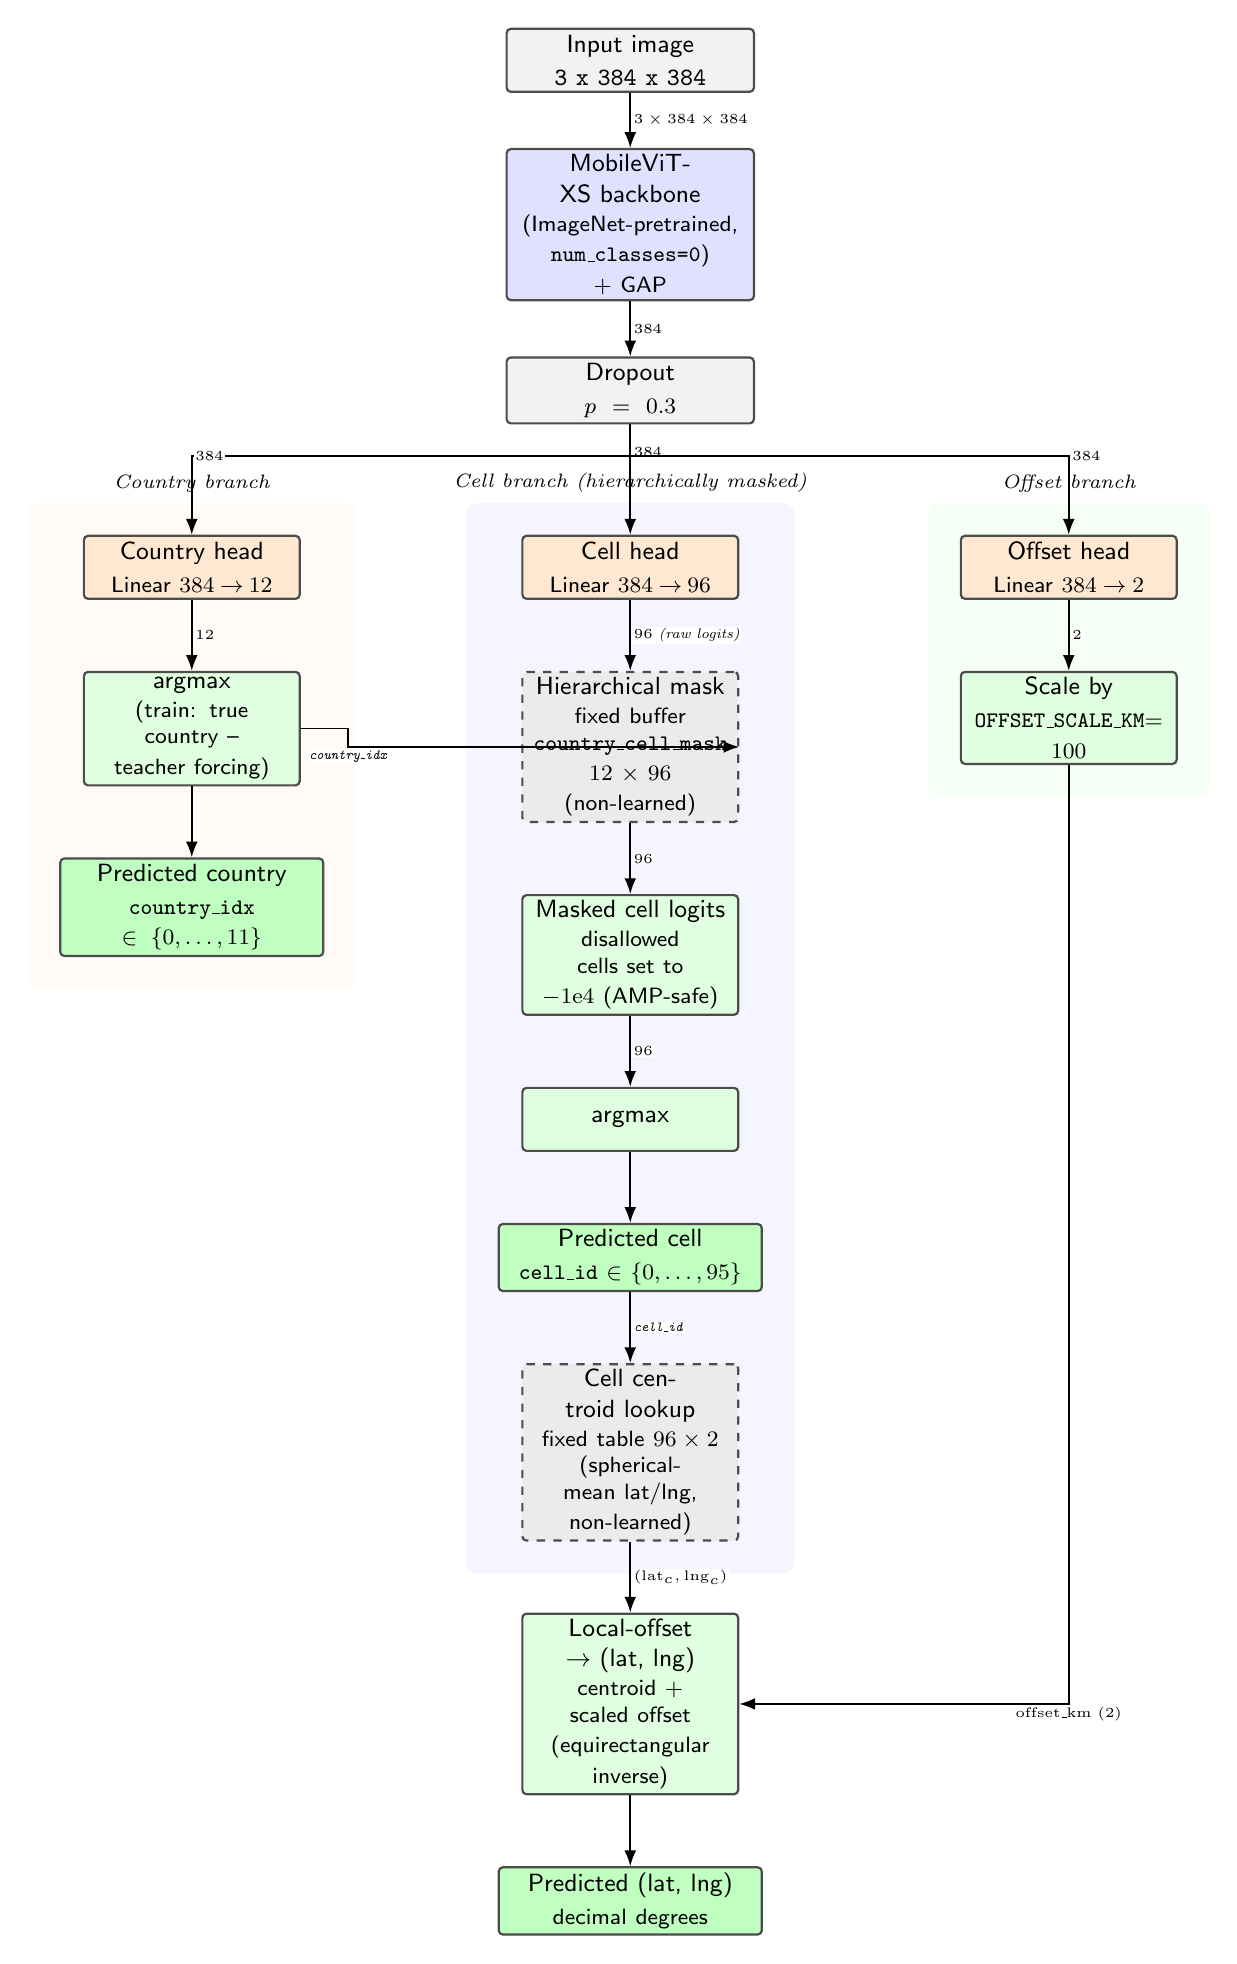
\begin{tikzpicture}[
  font=\sffamily\small,
  node distance=7mm and 12mm,
  >={Latex[length=2mm,width=1.5mm]},
  every path/.style={line width=0.6pt},
  block/.style={
    rectangle, rounded corners=1.5pt, draw=black!70, thick,
    minimum height=8mm, text width=30mm, align=center, inner sep=2pt
  },
  backbone/.style={block, fill=blue!12},
  head/.style={block, fill=orange!18, text width=26mm},
  fixed/.style={block, fill=black!8, dashed, text width=26mm},
  op/.style={block, fill=green!12, text width=26mm},
  outnode/.style={block, fill=green!25, thick, text width=32mm},
  % NOT sloped: rotated labels on short vertical connector arrows (most of this diagram)
  % overran into the neighboring boxes' text -- caught on the first render. Side-placed,
  % unrotated, tiny labels stay clear regardless of how short the arrow is.
  dimlabel/.style={font=\tiny\itshape, pos=0.5, right=0.5pt, fill=white, inner sep=0.5pt},
  dimlabelb/.style={font=\tiny\itshape, pos=0.5, below=0.5pt, fill=white, inner sep=0.5pt},
]

% ---- input / backbone / trunk ----
\node[block, fill=black!5] (input) {Input image\\[1pt]\texttt{3 x 384 x 384}};
\node[backbone, below=of input] (backbone) {MobileViT-XS backbone\\[1pt]\footnotesize(ImageNet-pretrained,\\ \texttt{num\_classes=0}) + GAP};
\node[block, fill=black!5, below=of backbone] (dropout) {Dropout\\[1pt]\footnotesize $p=0.3$};

\draw[->] (input) -- (backbone) node[dimlabel]{$3\times384\times384$};
\draw[->] (backbone) -- (dropout) node[dimlabel]{$384$};

% ---- three heads off the shared 384-d feature ----
\node[head, below left=14mm and 26mm of dropout] (country_head) {Country head\\[1pt]\footnotesize Linear $384\!\to\!12$};
\node[head, below=14mm of dropout] (cell_head) {Cell head\\[1pt]\footnotesize Linear $384\!\to\!96$};
\node[head, below right=14mm and 26mm of dropout] (offset_head) {Offset head\\[1pt]\footnotesize Linear $384\!\to\!2$};

\draw[->] (dropout.south) -- ++(0,-4mm) -| (country_head.north) node[pos=0.25,dimlabel]{$384$};
\draw[->] (dropout) -- (cell_head) node[dimlabel, pos=0.25]{$384$};
\draw[->] (dropout.south) -- ++(0,-4mm) -| (offset_head.north) node[pos=0.25,dimlabel]{$384$};

% ---- country branch: argmax / teacher forcing ----
\node[op, below=9mm of country_head] (country_argmax) {argmax\\[1pt]\footnotesize (train: true country --\\ teacher forcing)};
\draw[->] (country_head) -- (country_argmax) node[dimlabel]{$12$};
\node[outnode, below=9mm of country_argmax] (country_out) {Predicted country\\[1pt]\footnotesize \texttt{country\_idx} $\in\{0,\dots,11\}$};
\draw[->] (country_argmax) -- (country_out);

% ---- hierarchical mask: fixed (12 x 96) buffer combines country_idx with raw cell logits ----
\node[fixed, below=9mm of cell_head] (mask) {Hierarchical mask\\[1pt]\footnotesize fixed buffer \texttt{country\_cell\_mask}\\ $12\times96$ (non-learned)};
\draw[->] (cell_head) -- (mask) node[dimlabel]{$96$ (raw logits)};
\draw[->] (country_argmax.east) -- ++(6mm,0) |- (mask.east) node[pos=0.75, dimlabelb]{\texttt{country\_idx}};

\node[op, below=9mm of mask] (masked_logits) {Masked cell logits\\[1pt]\footnotesize disallowed cells set to\\ $-1\mathrm{e}{4}$ (AMP-safe)};
\draw[->] (mask) -- (masked_logits) node[dimlabel]{$96$};

\node[op, below=9mm of masked_logits] (cell_argmax) {argmax};
\draw[->] (masked_logits) -- (cell_argmax) node[dimlabel]{$96$};

\node[outnode, below=9mm of cell_argmax] (cell_out) {Predicted cell\\[1pt]\footnotesize \texttt{cell\_id} $\in\{0,\dots,95\}$};
\draw[->] (cell_argmax) -- (cell_out);

\node[fixed, below=9mm of cell_out] (centroid_lookup) {Cell centroid lookup\\[1pt]\footnotesize fixed table $96\times2$\\ (spherical-mean lat/lng,\\ non-learned)};
\draw[->] (cell_out) -- (centroid_lookup) node[dimlabel]{\texttt{cell\_id}};

% ---- offset branch: scale ----
\node[op, below=9mm of offset_head] (offset_scale) {Scale by\\[1pt]\footnotesize \texttt{OFFSET\_SCALE\_KM}$=100$};
\draw[->] (offset_head) -- (offset_scale) node[dimlabel]{$2$};

% ---- combine centroid + offset (below the LOWEST node of the cell branch, i.e. after
% centroid_lookup, not masked_logits -- getting this anchor wrong caused an overlap in an
% earlier draft) ----
\node[op, below=9mm of centroid_lookup] (combine) {Local-offset $\to$ (lat, lng)\\[1pt]\footnotesize centroid $+$ scaled offset\\ (equirectangular inverse)};

\draw[->] (centroid_lookup) -- (combine) node[dimlabel]{$(\mathrm{lat}_c,\mathrm{lng}_c)$};
\draw[->] (offset_scale.south) |- (combine.east) node[pos=0.8, dimlabelb]{$\mathrm{offset\_km}\ (2)$};

\node[outnode, below=9mm of combine] (final) {Predicted (lat, lng)\\[1pt]\footnotesize decimal degrees};
\draw[->] (combine) -- (final);

% ---- background grouping boxes ----
\begin{scope}[on background layer]
  \node[fit=(country_head)(country_argmax)(country_out), fill=orange!4, rounded corners=4pt, inner sep=4mm, label={[font=\scriptsize\itshape]above:Country branch}] {};
  \node[fit=(cell_head)(mask)(masked_logits)(cell_argmax)(cell_out)(centroid_lookup), fill=blue!4, rounded corners=4pt, inner sep=4mm, label={[font=\scriptsize\itshape]above:Cell branch (hierarchically masked)}] {};
  \node[fit=(offset_head)(offset_scale), fill=green!4, rounded corners=4pt, inner sep=4mm, label={[font=\scriptsize\itshape]above:Offset branch}] {};
\end{scope}

\end{tikzpicture}
\end{document}

% ---------------------------------------------------------------------------------------
% Params (verified via src/protocol/param_check.py):
%   backbone (MobileViT-XS)  1,932,848
%   country head (384->12)        4,620
%   cell head    (384->96)       36,960   (approx; head total below is exact)
%   offset head  (384->2)           770
%   total heads                  42,350
%   TOTAL                     1,975,198   / 5,000,000 budget (well under 4M, ~2M unused)
%
% Fold-0 screen result (2026-08-19, job 4043929, 100 epochs): best val median 225.3km
% (epoch 85), country acc 72.7%, cell acc 37.3%, <200km 46.0%, <750km 77.3%.
% ---------------------------------------------------------------------------------------
